% 等腰梯形性质：两腰相等 + 对角线相等 + 对称轴
\documentclass[tikz,border=4pt]{standalone}
\usepackage{ctex}
\usepackage{amsmath}
\usetikzlibrary{calc, decorations.markings}
\begin{document}
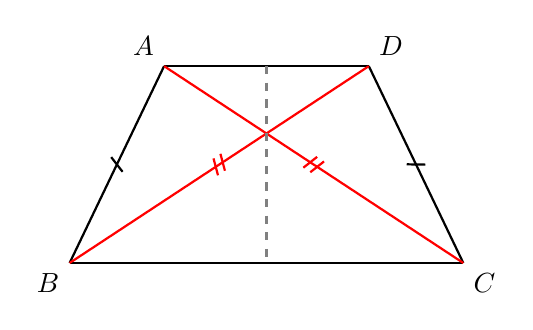
\begin{tikzpicture}[
  scale=1.0, thick,
  tickone/.style={postaction={decorate, decoration={markings,
    mark=at position 0.5 with {\draw (-1.5pt,-3pt) -- (1.5pt,3pt);}}}},
  ticktwo/.style={postaction={decorate, decoration={markings,
    mark=at position 0.5 with {\draw (-2.5pt,-3pt) -- (-0.5pt,3pt);
                               \draw (0.5pt,-3pt)  -- (2.5pt,3pt);}}}},
]
  \coordinate (A) at (1.2,2.5);
  \coordinate (D) at (3.8,2.5);
  \coordinate (B) at (0,0);
  \coordinate (C) at (5,0);
  \coordinate (M) at (2.5,2.5);
  \coordinate (N) at (2.5,0);

  \draw[tickone] (A)--(B);
  \draw[tickone] (D)--(C);
  \draw (A)--(D);
  \draw (B)--(C);

  % 对角线（红色，双划等长标记）
  \draw[red, ticktwo] (A)--(C);
  \draw[red, ticktwo] (B)--(D);

  % 对称轴（虚线）
  \draw[gray, dashed] (M)--(N);

  \node[above left]  at (A) {$A$};
  \node[above right] at (D) {$D$};
  \node[below left]  at (B) {$B$};
  \node[below right] at (C) {$C$};
\end{tikzpicture}
\end{document}
